% !TEX encoding = UTF-8
% !TEX TS-program = pdflatex
% !TEX root = ../tesi.tex

%**************************************************************
\chapter{Progettazione e codifica}
\label{ch:progettazione-e-codifica}
%**************************************************************

\intro{In questo capitolo vengono presentate le tecnologie e gli strumenti utilizzati, il ciclo di sviluppo del software adottato e i design pattern utilizzati.}\\

%**************************************************************
\section{Tecnologie}\label{sec:tecnologie}

Di seguito viene data una panoramica delle tecnologie e degli strumenti utilizzati.

\subsection*{CFR - decompilatore java}
CFR è il decompilatore utilizzato per trasformare il codice bytecode \textit{.class} in codice sorgente \textit{.java};
\url{http://www.benf.org/other/cfr/index.html}

\subsection*{Apk Tool}
Apktool è un tool per effettuare il reverse engineering delle applicazioni Android. Può decodificare le risorse contenute nell'APK in una forma quasi uguale a quelli originali, può anche di ricostruire l'APK dopo le modifiche alle risorse modificate.
\url{https://ibotpeaches.github.io/Apktool/}
\subsection*{Dex2Jar}
Questo strumento permette di trasformare i file \textit{.dex} in formato \textit{.jar} in modo che possa essere letta attraverso un software di compressione, come 7Zip, per poter accedere quindi ai file di tipo \textit{.class}.
\url{https://github.com/pxb1988/dex2jar}


\subsection*{Java}
In informatica, Java è un linguaggio di programmazione ad alto livello, orientato agli oggetti e tipizzazione statica, che si appoggia sull'omonima piattaforma software di esecuzione, specificamente progettato per essere il più possibile indipendente dalla piattaforma hardware di esecuzione.
\subsection*{Json}
JSON (JavaScript Object Notation) è un semplice formato per lo scambio di dati.
Per le persone è facile da leggere e scrivere, mentre per le macchine risulta facile da generare e analizzarne la sintassi.
JSON è basato su due strutture:
\begin{itemize}
    \item un insieme di coppie nome/valore, in diversi linguaggi, questo è realizzato come un oggetto, un record, uno struct, un dizionario, una tabella hash, un elenco di chiavi o un array associativo.
    \item un elenco ordinato di valori, nella maggior parte dei linguaggi questo si realizza con un array, un vettore o una sequenza.
\end{itemize}
\url{https://www.json.org/json-it.html}

\subsection*{XPath}\label{subsec:xpath}
In informatica XPath è un linguaggio, parte della famiglia XML, che permette di individuare i nodi all'interno di un documento XML. Le espressioni XPath, a differenza delle espressioni XML, non servono a identificare la struttura di un documento, bensì a localizzarne con precisione i nodi.


\section{Strumenti}\label{sec:strumenti}

\subsection*{Intellij IDEA}
L'IDE utilizzato per la scrittura del codice in Java sviluppato da JetBrains.
\url{https://www.jetbrains.com/idea/}

\subsection*{Android Emulator}
Lo strumento che permette di avviare degli emulatori Android, conosciuti anche come AVD. È stato utilizzato per eseguire l'applicazione ricompilata, per poter fare il dump dei dati presenti nell'area di storage dell'applicazione, come i file JSON, XML e SQLite, o come il file delle attività di rete.
\url{https://developer.android.com/studio/run/emulator}

\subsection*{Maven}
Maven è un tool di build automation, basato sul concetto di Project Object Model (POM), maven può gestire i build, fare il report e la documentazione da un singolo centro di informazione.
\url{https://maven.apache.org/}

\subsection*{Astah}
Astah è uno strumento di modellazione UML. Permette di creare vari diagrammi UML, come quelli di classe, di package, di sequenza e di attività.
\url{https://astah.net/products/astah-community/}

\subsection*{Git - GitLab}
Gitlab è una piattaforma web open-source che permette la gestione di repository e di funzioni d'issue tracking system.
Questa è un'istanza privata dell'azienda Imola Informatica S.p.A.
\url{https://git.imolinfo.it/users/sign_in}
%**************************************************************
\section{Ciclo di vita del software}\label{sec:ciclo-vita-software}
Il modello adottato per lo sviluppo del progetto è il modello incrementale, permettendo così di suddividere la durata del progetto in diversi incrementi, in ognuno dei quali sono stati definiti degli obiettivi/requisiti da raggiungere.
Inoltre, tale modello di sviluppo ha come conseguenza i seguenti vantaggi:
\begin{itemize}
    \item assegnare diverse priorità agli obiettivi da raggiungere, in modo che quelli più importanti vengano raggiunti prima;
    \item è possibile mostrare il prodotto al termine di ogni incremento in questo modo si assicura che il risultato di ogni incremento sia consono alle aspettative del cliente;
    \item la fase di verifica avviene ad ogni incremento in modo da garantire la correttezza del prodotto di ogni incremento;
    \item a ogni incremento vengono aggiunte delle funzionalità corrette e funzionanti, allora il prodotto finale soddisfa i requisiti del cliente;
\end{itemize}
%**************************************************************
\section{Progettazione}
\label{sec:progettazione}

\subsection{Package}\label{subsec:package}
Questo è il root package del tool, contiene altri package e le due classi elencati successivamente.
\begin{namespacedesc}
    \classdesc{ApatLauncher}{È la classe di launcher del tool, si occupa principalmente di mettere in relazione di observed-observer i componenti della vista con i dati del modello;}
    \classdesc{Utils}{La classe di utilities che ha delle funzioni statiche utilizzata nel tool per evitare la ripetizione del codice.}
\end{namespacedesc}

\subsubsection{Package it.imolinfo.apat.controller} %**************************
Questo è il package che contiene la classe Controller e ciò che riguarda l'interazione del controller con il filesystem.
\begin{namespacedesc}
    \classdesc{AndroidManifestEditor.java}{È la classe che si occupa, dato un oggetto di tipo File Android Manifest, di modificare e/o aggiungere il tag \textit{debugabble} impostando il suo valore a \textit{true};}
    \classdesc{Controller}{È il controller del MVC, si occupa di effettuare le operazioni di decompilazione, ricompilazione, decodifica e analisi dei file;}
    \classdesc{MVCModule}{È la classe di effettuare la dependency injection per la creazione del MVC.}
\end{namespacedesc}

\subsubsection{Package it.imolinfo.apat.model} %**************************
Questo package contiene le classi che riguardano il modello del pattern Model View Controller.
\begin{namespacedesc}
    \classdesc{Modello}{La classe che contiene i dati utili al corretto funzionamento del tool;}
    \classdesc{ModelState}{È la classe che viene usato per poter salvare lo stato del funzionamento del tool. Lo stato viene salvato quando viene chiuso il tool, e viene ricaricato al successivo avvio;}
    \classdesc{PDFWriter}{È la classe wrapper che si occupa della creazione del file PDF per salvare i risultati dell'analisi;}
    \classdesc{Result}{È la classe di messaggio che viene restituita quando il tool interagisce con il file system;}
    \classdesc{Unzipper}{È la classe si occupa di decomprimere i file zip;}
    \classdesc{Dumper}{È la classe che si occupa di effettuare il dump dei dati da un file con estensione \textit{db};}
\end{namespacedesc}

\subsubsection{Package it.imolinfo.apat.pattern} %**************************
Questo package contiene degli sotto-package ognuno dei quali rappresenta un design pattern utilizzato nello sviluppo del tool.
I pattern utilizzati sono
\begin{namespacedesc}
    \classdesc{analyzer.Analyze}{È l'interfaccia di base del pattern Decorator.}
    \classdesc{analyzer.BaseAnalyzer}{È la classe dell'oggetto base che viene decorato.}
    \classdesc{analyzer.BaseAnalyzeDecorator}{È il classe astratta del decorator di base che implementa l'interfaccia Analyze, e ha un metodo astratto \textit{doAnalysis()} che deve essere implementato dai decorator concreti.}
    \classdesc{analyzer.DumpDataBase}{È il decorator che si occupa di estrarre i contenuti dei file \textit{.db} scaricati dall'area di storage dell'app.}
    \classdesc{analyzer.DumpedFilesAnalyzer}{È il decorator che si occupa di analizzare i file dell'area di storage dell'applicazione con estensione \textit{XML} e \textit{json}, principalmente, legge il contenuto di tali file, e in base ad una whitelist, seleziona quali risultati restituire al chiamante.}
    \classdesc{analyzer.LambdaCounter}{È il decorator che conta il numero di lambda presente per ogni classe di codice \textit{.java} decompilato.}
    \classdesc{analyzer.StringFinder}{È il decorator che analizza i file di tipo \textit{.java}, ed estrae le stringhe hardcoded, può essere utilizzato insieme a un blacklist delle stringhe che devono essere ignorate.}
\end{namespacedesc}
\begin{namespacedesc}
    \classdesc{observer.Observable}{La classe parametrizzata T che può essere osservato;}
    \classdesc{observer.Observer}{L'interfaccia parametrizzata che ha il ruolo dell'observer;}
\end{namespacedesc}
\begin{namespacedesc}
    \classdesc{CliCommandFactory.Commands}{È l'interfaccia che contiene i metodi, dove ognuno dei quali deve generare delle istruzioni per la linea di comando.}
    \classdesc{CliCommandFactory.CommandFactory}{È la classe astratta che implementa la precendente interfaccia, con un costruttore di base che richiede un path di base.}
    \classdesc{CliCommandFactory.UnixCommandFactory}{È l'implementazione della classe astratta CommandFactory per il sistema UNIX.}
    \classdesc{CliCommandFactory.WindowsCommandFactory}{È l'implementazione della classe astratta CommandFactory per il sistema Windows.}
\end{namespacedesc}

\subsubsection{Package it.imolinfo.apat.view} %**************************
\begin{namespacedesc}
    \classdesc{AnalysisChooser}{È la finestra che mostra le opzioni di analisi.}
    \classdesc{View}{È la finestra principale, dove permette di selezionare il file \textit{apk} da decompilare ed analizzare.}
    \classdesc{WaitAction}{È una classe astratta che a sua volta eredita dalla classe Action e permette di eseguire un processo mostrando la barra del caricamento.}
    \classdesc{ApkFilter}{È l'implementazione dell'interfaccia \textbf{FileFilter} che accetta solo i file di tipo \textit{APK}.}
    \classdesc{KeyStoreFilter}{È l'implementazione dell'interfaccia \textbf{FileFilter} che accetta solo i file di tipo \textit{JKS}.}
    \classdesc{TextFilter}{È l'implementazione dell'interfaccia \textbf{FileFilter} che accetta solo i file di tipo \textit{txt}.}
\end{namespacedesc}


%**************************************************************

\section{Design Pattern utilizzati}\label{sec:design-pattern-utilizzati}
Di seguito, sono elencati i design pattern utilizzati durante la creazione del tool. Per ognuno di questi, verrà fornito il diagramma delle classi e una descrizione.
\subsection*{Model View Controller}\label{subsec:model-view-controller}
Come pattern architetturale è stato adottato il pattern Model-View-Controller, poiché è in grado di separare la logica di presentazione dei dati dalla logica di business.
\begin{figure}[H]
    \centering
    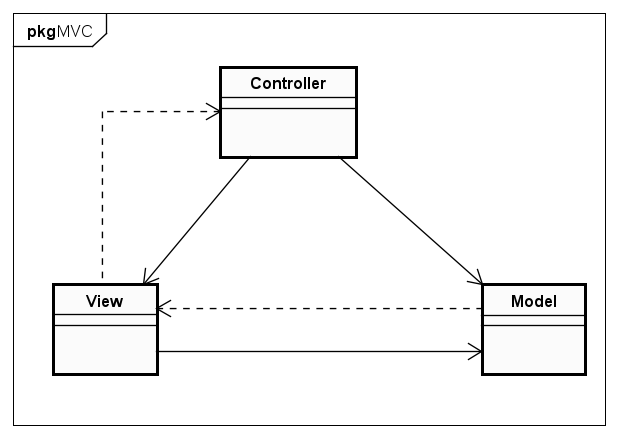
\includegraphics[width=14cm, height=8cm]{./immagini/diagrammi_uml/mvc.png}
    \caption{Diagramma delle classi del pattern MVC}\label{fig:mvc}
\end{figure}
\subsection*{Observer}\label{subsec:observer}
Il pattern observer permette di definire una dipendenza uno a molti fra oggetti, in modo tale che se un oggetto cambia il suo stato, tutti gli oggetti dipendenti da questo siano notificati e aggiornati automaticamente.\\
Tale pattern viene applicato nel tool perché i componenti delle viste possano osservare il contenuto del modello.
\begin{figure}[H]
    \centering
    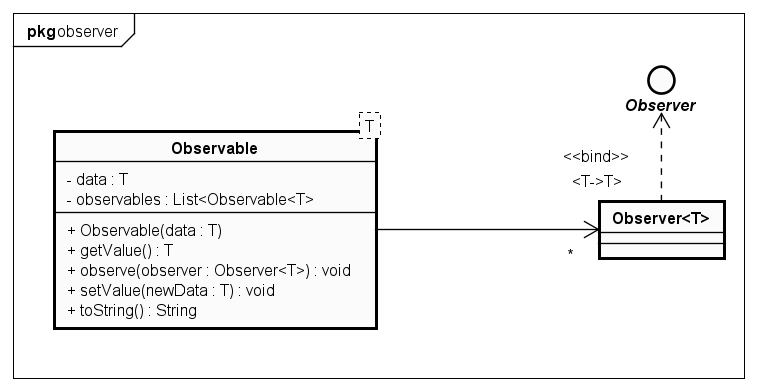
\includegraphics[width=13cm, height=8cm]{./immagini/diagrammi_uml/Observer.png}
    \caption{Diagramma delle classi del pattern Observer}\label{fig:observer}
\end{figure}
\subsection*{Decorator}\label{subsec:decorator}
Il pattern decorator è stato utilizzato per creare la parte del tool che si occupa di effettuare l'analisi del codice decompilato e dei file scaricati dall'area di storage dell'applicazione presenti nell'Android Emulator Device.
Il vantaggio ottenuto per aver utilizzato questo pattern è quello di poter "decorare" l'oggetto base di analisi, ovvero l'istanza della classe \textit{BaseAnalyzer} con i vari decorator, un altro importante vantaggio è quello di poter aggiungere altre funzionalità di analisi facilmente nel tool, infatti, è sufficiente creare un'altra sottoclasse della classe \textit{BaseAnalyzeDecorator} quindi implementare il metodo astratto.
\begin{figure}[H]
    \centering
    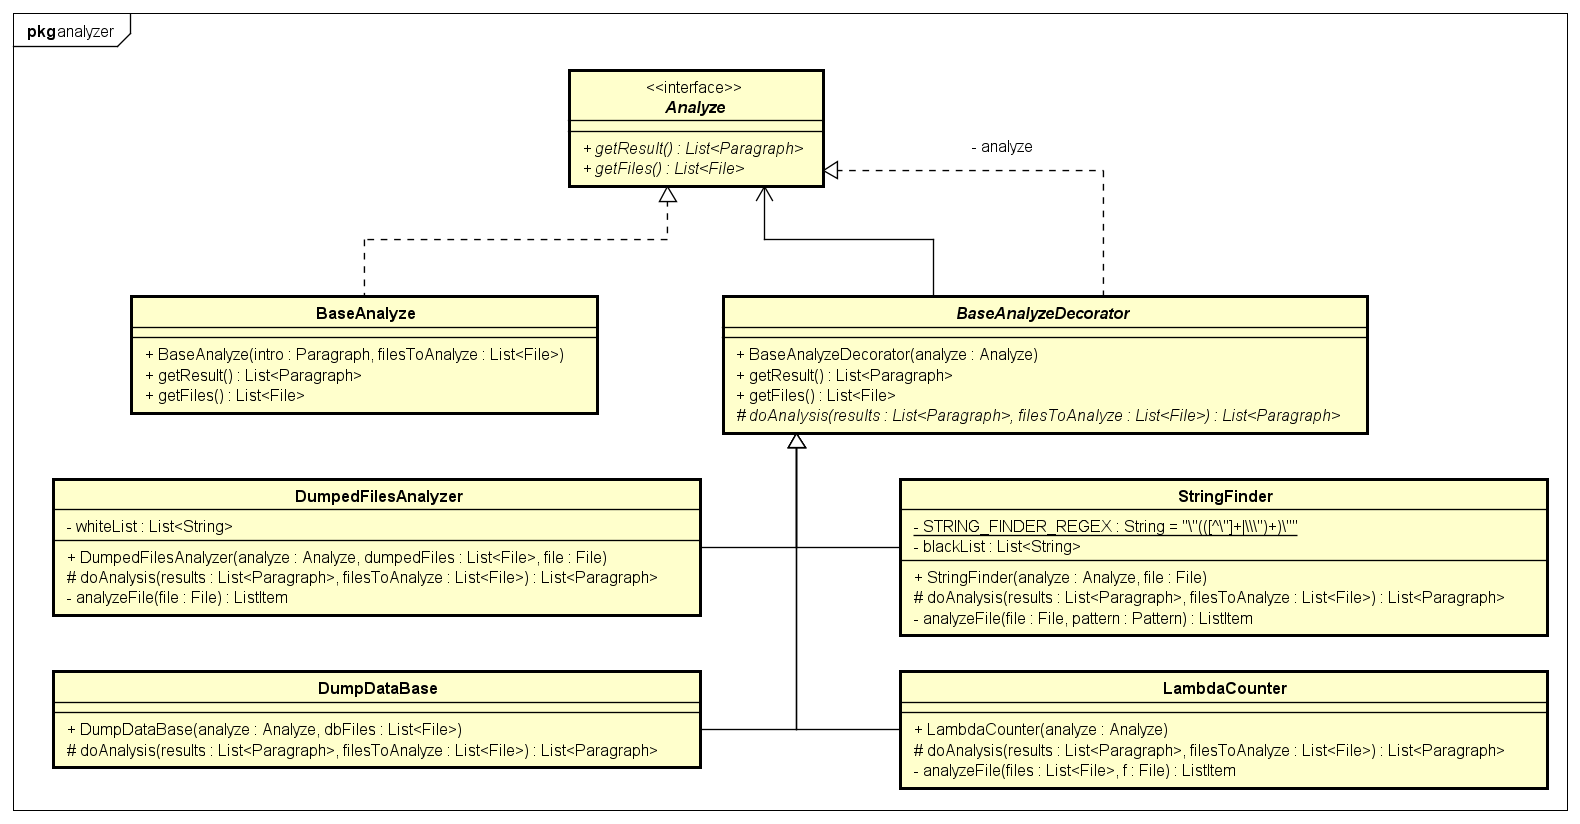
\includegraphics[width=13cm, height=10cm]{./immagini/diagrammi_uml/Decorator.png}
    \caption{Diagramma delle classi del pattern Decorator}\label{fig:decorator}
\end{figure}

\subsection*{Factory Method}\label{subsec:factory-method}
Questo pattern è stato utilizzato per poter fornire al controller dei comandi da eseguire nei processi, essendo i comandi dipendente dal sistema operativo, sono state create due classi, una per Windows chiamata \textit{WindowsCommandFactory} e una per Linux chiamata \textit{LinuxCommandFactory}.
Allo start-up del tool, viene letta una dalla JVM una variabile chiamata \textit{os.name}, e dipendentemente da valore letto, viene deciso quale delle sottoclassi istanziare per il corretto funzionamento del tool.
\begin{figure}[H]
    \centering
    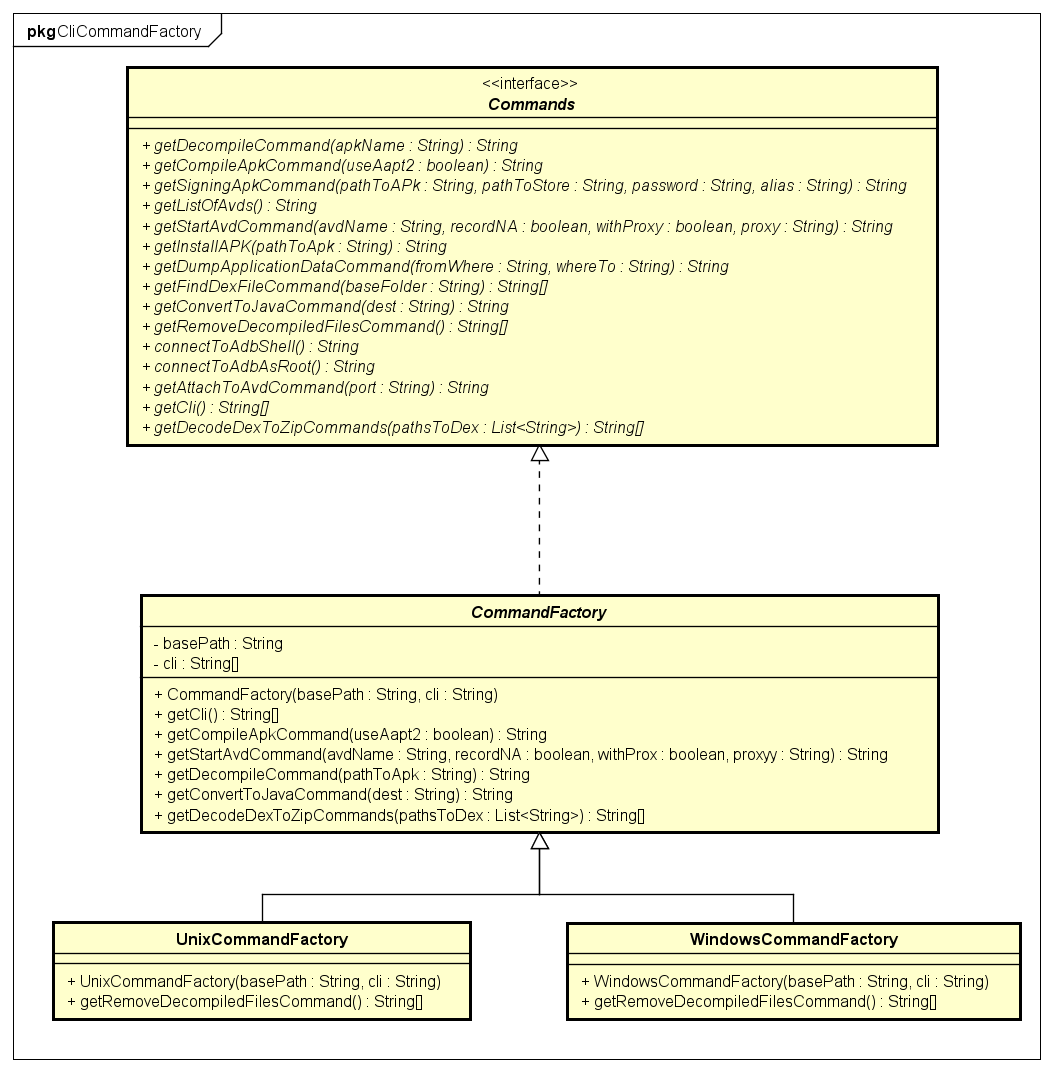
\includegraphics[width=14cm, height=12cm]{./immagini/diagrammi_uml/CommandFactory.png}
    \caption{Diagramma delle classi del pattern FactoryMethod}\label{fig:factory-method}
\end{figure}
%**************************************************************
\section{Codifica}\label{sec:codifica}
